\documentclass{article}

\usepackage[english]{babel}

\usepackage[letterpaper,top=2cm,bottom=2cm,left=3cm,right=3cm,marginparwidth=1.75cm]{geometry}
\usepackage{robust-externalize}
\usepackage{subcaption}
\robExtConfigure{enable fallback to manual mode} % Optional, but prints instructions if shell-escape is disabled instead of giving a compilation error.

\usepackage{amsmath}
\usepackage{graphicx}
\usepackage[colorlinks=true, allcolors=blue]{hyperref}
\usepackage{array}

\title{Movies Dataset Report}
\author{Akshat Shukla}

\begin{document}
\maketitle

\begin{abstract}
An analysis on the Song dataset provided by KDAG, IIT Kharagpur as a part of their Selection Process
\end{abstract}

\section{Generate vectors for the three keywords}
\subsection{Dataset overview}
The dataset we are provided with has the following columns:
\begin{itemize}
    \item Song ID
    \item Genre (GT Values)
    \item keyword1
    \item keyword2
    \item keyword3
\end{itemize}
\begin{table}[h]
\centering
\begin{tabular}{|c|c|c|c|c|}
    \hline
    \textbf{Song ID} & \textbf{Genre (GT Values)} & \textbf{keyword1} & \textbf{keyword2} & \textbf{keyword3} \\
    \hline
    74 & guitar & happy & distorted & rock \\
    103 & brass & energetic & melodic & classical \\
    201 & banjo & happy & acoustic & country \\
    194 & synth & energetic & heavy & hip-hop \\
    184 & synth & energetic & slow & hip-hop \\
    97 & brass & calm & upbeat & classical \\
    63 & guitar & energetic & melodic & rock \\
    ... & ... & ... & ... & ... \\
    \hline
\end{tabular}
\caption{Head of our dataframe}
\label{fig:head_of_dataframe}
\end{table}

These keywords correspond to different aspects of the song. We will generate vectors for these keywords using the LF-IDF method as well as the Bag of words method.

\begin{table}[h]
\centering
\begin{minipage}{0.3\textwidth}
\centering
\begin{tabular}{|l|r|}
    \hline
    \multicolumn{2}{|c|}{\textbf{keyword\_1}} \\
    \hline
    guitar & 65 \\
    synth & 43 \\
    piano & 12 \\
    brass & 11 \\
    violin & 10 \\
    banjo & 6 \\
    \hline
    \multicolumn{2}{|c|}{Name: count, dtype: int64} \\
    \hline
\end{tabular}
\caption{Keyword 1 counts}
\label{tab:keyword1_counts}
\end{minipage}
\hfill
\begin{minipage}{0.3\textwidth}
\centering
\begin{tabular}{|l|r|}
    \hline
    \multicolumn{2}{|c|}{\textbf{keyword\_2}} \\
    \hline
    happy & 30 \\
    mellow & 28 \\
    energetic & 27 \\
    sad & 21 \\
    angry & 12 \\
    emotional & 11 \\
    calm & 11 \\
    upbeat & 4 \\
    nostalgic & 3 \\
    \hline
    \multicolumn{2}{|c|}{Name: count, dtype: int64} \\
    \hline
\end{tabular}
\caption{Keyword 2 counts}
\label{tab:keyword2_counts}
\end{minipage}
\hfill
\begin{minipage}{0.3\textwidth}
\centering
\begin{tabular}{|l|r|}
    \hline
    \multicolumn{2}{|c|}{\textbf{keyword\_3}} \\
    \hline
    fast & 28 \\
    melodic & 27 \\
    slow & 23 \\
    upbeat & 20 \\
    rhythmic & 14 \\
    heavy & 10 \\
    acoustic & 9 \\
    twangy & 6 \\
    distorted & 5 \\
    danceable & 5 \\
    \hline
    \multicolumn{2}{|c|}{Name: count, dtype: int64} \\
    \hline
\end{tabular}
\caption{Keyword 3 counts}
\label{tab:keyword3_counts}
\end{minipage}
\end{table}

for our use, the TF-IDF Embedding model captures more information since it takes into account the frequency of the words in the dataset. The Bag of Words model only captures the presence of the word in the dataset.
Since both of these correspond to embeddings with the same dimensions, the TD-IDF Model is considred for our use.

\subsection{Keyword Embedding Generation}
To generate the keyword embeddings, we will use the TF-IDF method. The TF-IDF (Term Frequency-Inverse Document Frequency) method helps in understanding the importance of a keyword in relation to the dataset.

\subsubsection{TF-IDF Calculation}
The TF-IDF value is calculated as follows:
\begin{equation}
\text{TF-IDF}(t, d) = \text{TF}(t, d) \times \text{IDF}(t)
\end{equation}
where:
\begin{itemize}
    \item $\text{TF}(t, d)$ is the term frequency of term $t$ in document $d$.
    \item $\text{IDF}(t)$ is the inverse document frequency of term $t$.
\end{itemize}
The term frequency (TF) is calculated as:
\begin{equation}
\text{TF}(t, d) = \frac{f_{t,d}}{\sum_{t' \in d} f_{t',d}}
\end{equation}
where $f_{t,d}$ is the frequency of term $t$ in document $d$.

The inverse document frequency (IDF) is calculated as:
\begin{equation}
\text{IDF}(t) = \log \left( \frac{N}{|\{d \in D : t \in d\}|} \right)
\end{equation}
where $N$ is the total number of documents and $|\{d \in D : t \in d\}|$ is the number of documents containing term $t$.

We generate the TF-IDF Bases Embeddings for each keyword in the dataset and store them for future use

\cite{word2vec_tfidf}
\begin{table}[h]
\centering
\begin{tabular}{|c|c|c|c|}
    \hline
    \textbf{Song ID} & \textbf{tf-idf-keyword1} & \textbf{tf-idf-keyword2} & \textbf{tf-idf-keyword3} \\
    \hline
    74 & [0., 0., 0.36, 0., 0., 0.] & [0., 0., 0., 0., 0.32, 0., \ldots] & [0., 0., 0.11, 0., 0., 0., \ldots] \\
    103 & [0., 0.19, 0., 0., 0., 0.] & [0., 0., 0., 0.31, 0., 0., \ldots] & [0., 0., 0., 0., 0., 0.31, \ldots] \\
    201 & [0.13, 0., 0., 0., 0., 0.] & [0., 0., 0., 0., 0.32, 0., \ldots] & [0.17, 0., 0., 0., 0., 0., \ldots] \\
    194 & [0., 0., 0., 0., 0.35, 0.] & [0., 0., 0., 0.31, 0., 0., \ldots] & [0., 0., 0., 0., 0.18, 0., \ldots] \\
    \ldots & \ldots & \ldots & \ldots \\
    \hline
\end{tabular}
\caption{Generated Embeddings}
\label{fig:head_of_dataframe}
\end{table}

\section{Dimensionality Reduction}
We will utilize Principal Component Analysis (PCA) on individual keywords in our dataset in order to reduce the dimensionality of the generated embeddings.

Via Princimple Component analysis, we find the directions along which the variance of the data is maximized and project the data onto these directions.

Thus, we can reduce the dimensionality of the data while retaining most of the information.

The Principle Component vectors are found as:
\begin{equation}
    \text{PCA}(X) = X \cdot V
\end{equation}
where $X$ is the standardized data matrix and $V$ is the matrix of eigenvectors of the covariance matrix of $X$.

We will use the first $2$ eigenvectors to reduce the dimensionality of the data.

\cite{pca_gfg}
\begin{table}[h]
    \centering
    \begin{tabular}{|c|c|c|c|c|c|c|}
        \hline
        \textbf{song\_id} & \textbf{kw1\_pca1} & \textbf{kw1\_pca2} & \textbf{kw2\_pca1} & \textbf{kw2\_pca2} & \textbf{kw3\_pca1} & \textbf{kw3\_pca2} \\
        \hline
        74 & 1.349694 & 0.370477 & -2.051477 & 0.344695 & -0.047019 & -0.192033 \\
        103 & -0.538837 & -1.813324 & 0.695438 & -1.910713 & -1.646868 & 1.482767 \\
        201 & -0.501082 & -1.376430 & -2.051477 & 0.344695 & -0.055551 & -0.233782 \\
        194 & -1.556300 & 1.033730 & 0.695438 & -1.910713 & -0.058292 & -0.247738 \\
        184 & -1.556300 & 1.033730 & 0.695438 & -1.910713 & -0.203708 & -1.817350 \\
        \hline
    \end{tabular}
    \caption{PCA values for keywords}
    \label{tab:pca_values}
\end{table}
We use \texttt{np.cov} in order to obtain the covariance matrix of the given standardized data and use \texttt{np.linalg.eigh} in order to obtain the eigenvectors of the covariance matrix

\section{Combining the Embeddings into one}
\subsection{Embedding Format}
Here, we choose a simple embedding for every datapoint: The embedding is a three dimensional vector consisting of the average PCA values of the three keywords for that datapoint.

This provides us with a three dimensional view of each datapoint based on the values of their individual keywords.
\begin{figure}[h]
\centering
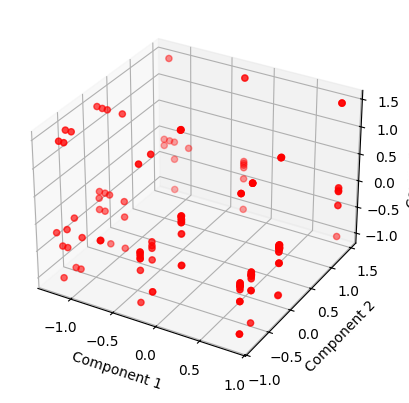
\includegraphics{output.png}
\caption{Visualization of the combined embeddings}
\label{fig:combined_embeddings}
\end{figure}

The Embeddings were plottted using desmos \href{https://www.desmos.com/3d/ui3zwls4ck}{here}

\section{Clustering}
Here, we utilize k means clustering in order to cluster the embeddings into different groups. Later, we find out the silhouette score for various values of embeddings and plot them.

We choose a value of \texttt{k = 8} since the points, plotted in 3d space could be deciphered visually into 8 clusters.

Later, We will use these clusters in order to predict the Genre (Ground Truth) values for new datapoints.

To Implement k-means clustering, we initialize \texttt{k = 8} points in the space and assign each point to the cluster with the nearest centroid. We then update the centroid of each cluster to be the mean of the points in that cluster. We repeat this process until the centroids converge.

After clustering, all points are assigned clusters. Here, we can infer that the points belonging to the same cluster have the same genre, with the mode of each cluster appearing more than half of the times.

\cite{kmeans_gfg}
\begin{figure}[h]
\centering
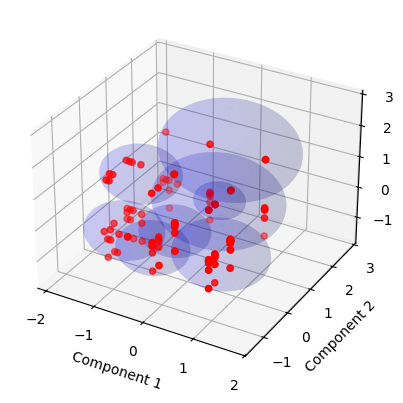
\includegraphics{output2.png}
\caption{Visualization for the final cluster assignment}
\label{fig:cluster_assignment}
\end{figure}

A more interactive simulation can be found over at desmos \href{https://www.desmos.com/3d/njmqmzwlyy}{here}

\section{Analysis}
\subsection{Ground Truth Distribution in clusters}
\begin{table}[h]
\centering
\begin{tabular}{|c|c|c|c|}
    \hline
    \textbf{Cluster Number} & \textbf{Modal Genre} & \textbf{\# Points} & \textbf{Percentage of Modal Genre} \\
    \hline
    0 & rock & 45 & 44.44 \\
    1 & rock & 22 & 22.73 \\
    2 & hip-hop & 15 & 66.67 \\
    3 & rock & 8 & 50.00 \\
    4 & hip-hop & 15 & 66.67 \\
    5 & classical & 14 & 50.00 \\
    6 & classical & 22 & 68.18 \\
    7 & pop & 6 & 33.33 \\
    \hline
\end{tabular}
\caption{Cluster Analysis}
\label{tab:cluster_analysis}
\end{table}

One comeback of this appreach is that we were unable to assign any clusters with the \texttt{country} genre as the modal one since the number of such datapoints do not appear to be close together in the 3d space.


Even though there are overlaps, we were able to seperate almost all the genres into different clusterings.
\subsection{Silhouette Score}
The silhouette score is a measure of how similar an object is to its own cluster (cohesion) compared to other clusters (separation). The silhouette ranges from -1 to 1, where a high value indicates that the object is well matched to its own cluster and poorly matched to neighboring clusters.

The silhouette score for a given clustering is given as:
\begin{equation}
    \text{Silhouette Score} = \frac{b - a}{\max(a, b)}
\end{equation}
where:
\begin{itemize}
    \item $a$ is the mean distance between a sample and all other points in the same class.
    \item $b$ is the mean distance between a sample and all other points in the next nearest cluster.
\end{itemize}
\cite{shilouette_gfg}

The total silhouette score is equal to the mean of all the silhouette scores of the individual clusters.

We plotted the Silhouette score for various values of k and found that the score kept increasing as the number of clusters increased. This is because the number of clusters increased, the points were more likely to be closer to their own cluster than to the next nearest cluster.

\begin{figure}[h]
\centering
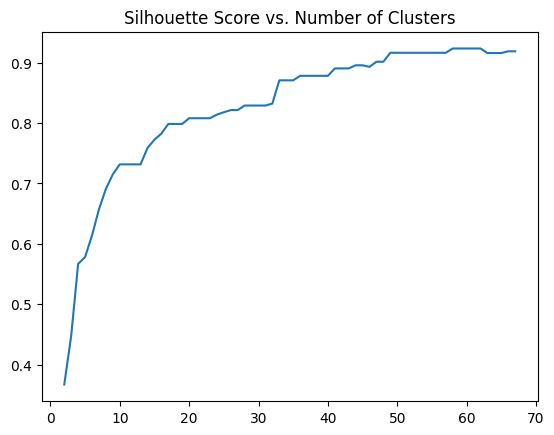
\includegraphics[width=300pt]{output3.png}
\caption{Silhouette Score for various values of k}
\label{fig:silhouette_score}
\end{figure}

\subsection{Assigning Genres to new datapoints}
\begin{itemize}
    \item In order to assign genres to new data, we perform exactly the same operations onto them as we did when generating embeddings for our original dataset, using the means and standard deviations of our original data set.
    \item We find out the closest cluster for this new data and assign the genre for the datapoint to be picked based on a binomial distribution on the genres present in the cluster 
\end{itemize}
\begin{table}[h]
\centering
\begin{tabular}{|c|c|c|c|c|c|}
    \hline
    \textbf{Point Number} & \textbf{Keyword 1} & \textbf{Keyword 2} & \textbf{Keyword 3} & \textbf{Closest Cluster} & \textbf{Assigned Genre} \\
    \hline
    0 & piano & calm & slow & 6 & classical \\
    1 & guitar & emotional & distorted & 0 & rock \\
    2 & synth & mellow & distorted & 1 & rock \\
    \hline
\end{tabular}
\caption{Assigning clusters to new datapoints}
\label{tab:point_assignment}
\end{table}

The assigned genres are: classical, country and rock respectively. which seem to be intuitive based on the keywords provided.

An interactive simulation can be viewed on desmos \href{https://www.desmos.com/3d/bqnuuli8ra}{here}

\section{Bonus}

\subsection{Extrinsic measures for clustering}

some of the extrinsic measures used for analyzing the validity of clustering are:

\begin{itemize}
    \item \textbf{The Fowlkes-Mallows index}
    It is defined as:
    \begin{equation}
        \text{FMI} = \frac{\text{TP}}{\sqrt{(\text{TP} + \text{FP}) \times (\text{TP} + \text{FN})}}
    \end{equation}
    where:
    \begin{itemize}
        \item TP is the number of true positives (pairs of points that are in the same cluster and in the same ground truth class).
        \item FP is the number of false positives (pairs of points that are in the same cluster but in different ground truth classes).
        \item FN is the number of false negatives (pairs of points that are in the same ground truth class but in different clusters).
    \end{itemize}
    \cite{fowlkes_mallows_wiki}
    \item \textbf{Rand Index}
    used to measure the similarity between the ground truth and the clustering. The Rand Index is defined as:
    \begin{equation}
        \text{RI} = \frac{\text{TP} + \text{TN}}{\text{TP} + \text{FP} + \text{FN} + \text{TN}}
    \end{equation}
    where:
    \begin{itemize}
        \item TP is the number of true positives (pairs of points that are in the same cluster and in the same ground truth class).
        \item FP is the number of false positives (pairs of points that are in the same cluster but in different ground truth classes).
        \item FN is the number of false negatives (pairs of points that are in the same ground truth class but in different clusters).
        \item TN is the number of true negatives (pairs of points that are in different clusters and in different ground truth classes).
    \end{itemize}
    \cite{rand_index_wiki}
\end{itemize}

Here, we utilize the Rand Index in order to find the similarity between the ground truth and the clustering. The Rand Index ranges from 0 to 1, where a value of 1 indicates that the clustering is identical to the ground truth.

The Rand Index is calculated using the labels predicted using a binomial distribution and ground truth labels. We obtain a Rand Index of \texttt{0.734} which indicates that the clustering replicates the ground truth to a large extent.

\begin{table}[h]
\centering
\begin{tabular}{|c|c|c|}
    \hline
    \textbf{song\_id} & \textbf{genre} & \textbf{assigned\_genre} \\
    \hline
    74 & rock & rock \\
    103 & classical & classical \\
    201 & country & pop \\
    194 & hip-hop & hip-hop \\
    184 & hip-hop & pop \\
    \hline
\end{tabular}
\caption{Comparison of Actual and Assigned Genres}
\label{tab:genre_comparison}
\end{table}

\subsection{Ingenious Embeddings for the keywords}
\begin{itemize}
    \item We utilize embedding by rank. The embedding for each keyword is a vector of length \texttt{6} where the value at each index corresponds to the rank of the keyword in the count of the keyword in the dataset.
    
    \item We find the optimal value of k by finding out the shilouette score at various values. I turns out that we have a local amxima at \texttt{k = 6} and thus we choose this value for our clustering.
    

    \begin{figure}[h]
    \centering
    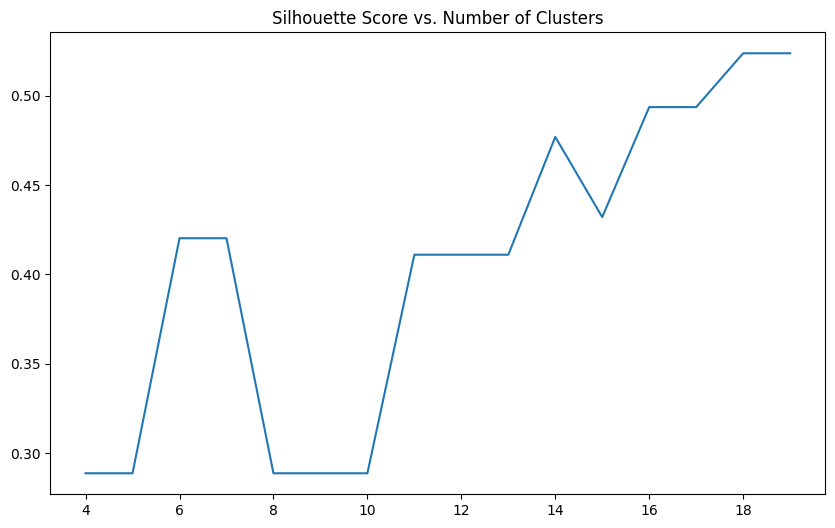
\includegraphics[width=400pt]{output4.png}
    \caption{Silhouette score for the clustering across various k}
    \label{fig:ingenious_embeddings}
    \end{figure}
    
    \item However, for this clustering, the Rand Index turns out to be \texttt{0.66} which is much worse than what we had achieved earlier. This clearly depicts the rquirement of a good embedding for the clustering to be successful.
    
    \item Visually, it is tough to seperate these embeddings into groups. The embeddings generated can be visualized \href{https://www.desmos.com/3d/xvcggpgx8i}{here}

    \item Clearly, Clustering based on the embeddings generated by the TF-IDF method is much better than the embeddings generated by the rank method.
\end{itemize}

\subsection{Further exploration of the Dataset}
\subsubsection{Analyzing the relation between genres and keywords}
\begin{itemize}
    \item Looking at the bar plot for Genre v/s Keyword 1, It becomes clear that the instrument being used largely affects the genre of the song.
    \item For example, all hip-hop make use of \texttt{synth}. All rock songs make use of \texttt{guitar}. Looking closely at the data, only classical songs make use of the \texttt{brass} or \texttt{violin}.
    \item Looking at Genre v/s Keyword 2, the separation is not very clear. However, some inferences can be drawn. For example, if a song is \texttt{upbeat}, it is more likely to be a \texttt{pop} song. If a song is \texttt{calm}, it is more likely to be a \texttt{classical} or a \texttt{pop} song.
\end{itemize}
\begin{figure}[h]
    \centering
    \begin{subfigure}[b]{0.3\textwidth}
        \centering
        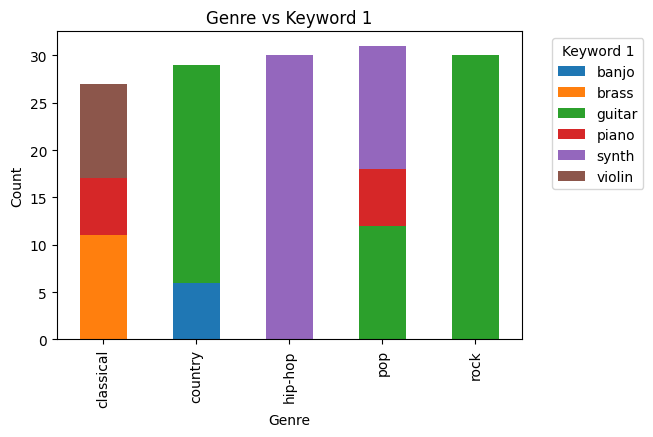
\includegraphics[width=\textwidth]{output5.png}
        \caption{Genre vs Keyword 1}
        \label{fig:genre_keyword1}
    \end{subfigure}
    \hfill
    \begin{subfigure}[b]{0.3\textwidth}
        \centering
        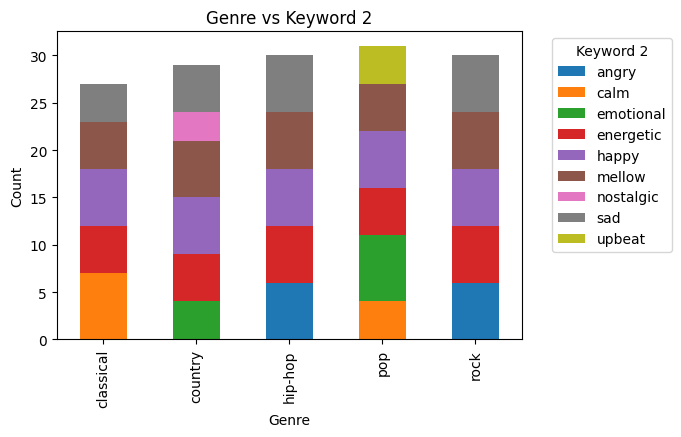
\includegraphics[width=\textwidth]{output6.png}
        \caption{Genre vs Keyword 2}
        \label{fig:genre_keyword2}
    \end{subfigure}
    \hfill
    \begin{subfigure}[b]{0.3\textwidth}
        \centering
        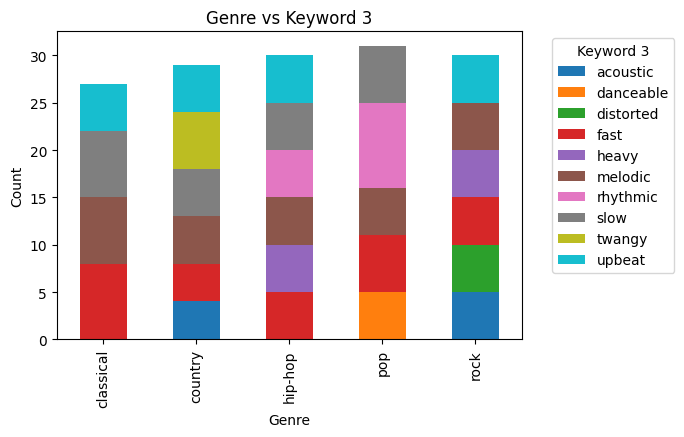
\includegraphics[width=\textwidth]{output7.png}
        \caption{Genre vs Keyword 3}
        \label{fig:genre_keyword3}
    \end{subfigure}
    \caption{Analysis of Genre vs Keywords}
    \label{fig:genre_keywords}
\end{figure}

\subsubsection{Analyzing the Correlation between Keywords and genres}
\begin{itemize}
    \item The Correlation matrix for the keywords and genres brings out similar inferences as were drawn from the bar plots.
    \item For example, \texttt{guitar} and \texttt{rock} have a high correlation of \texttt{0.57}. Moreover, \texttt{hip-hop} and \texttt{synth} have The highest correlation of \texttt{0.79}.
\end{itemize}
\begin{figure}[h]
    \centering
    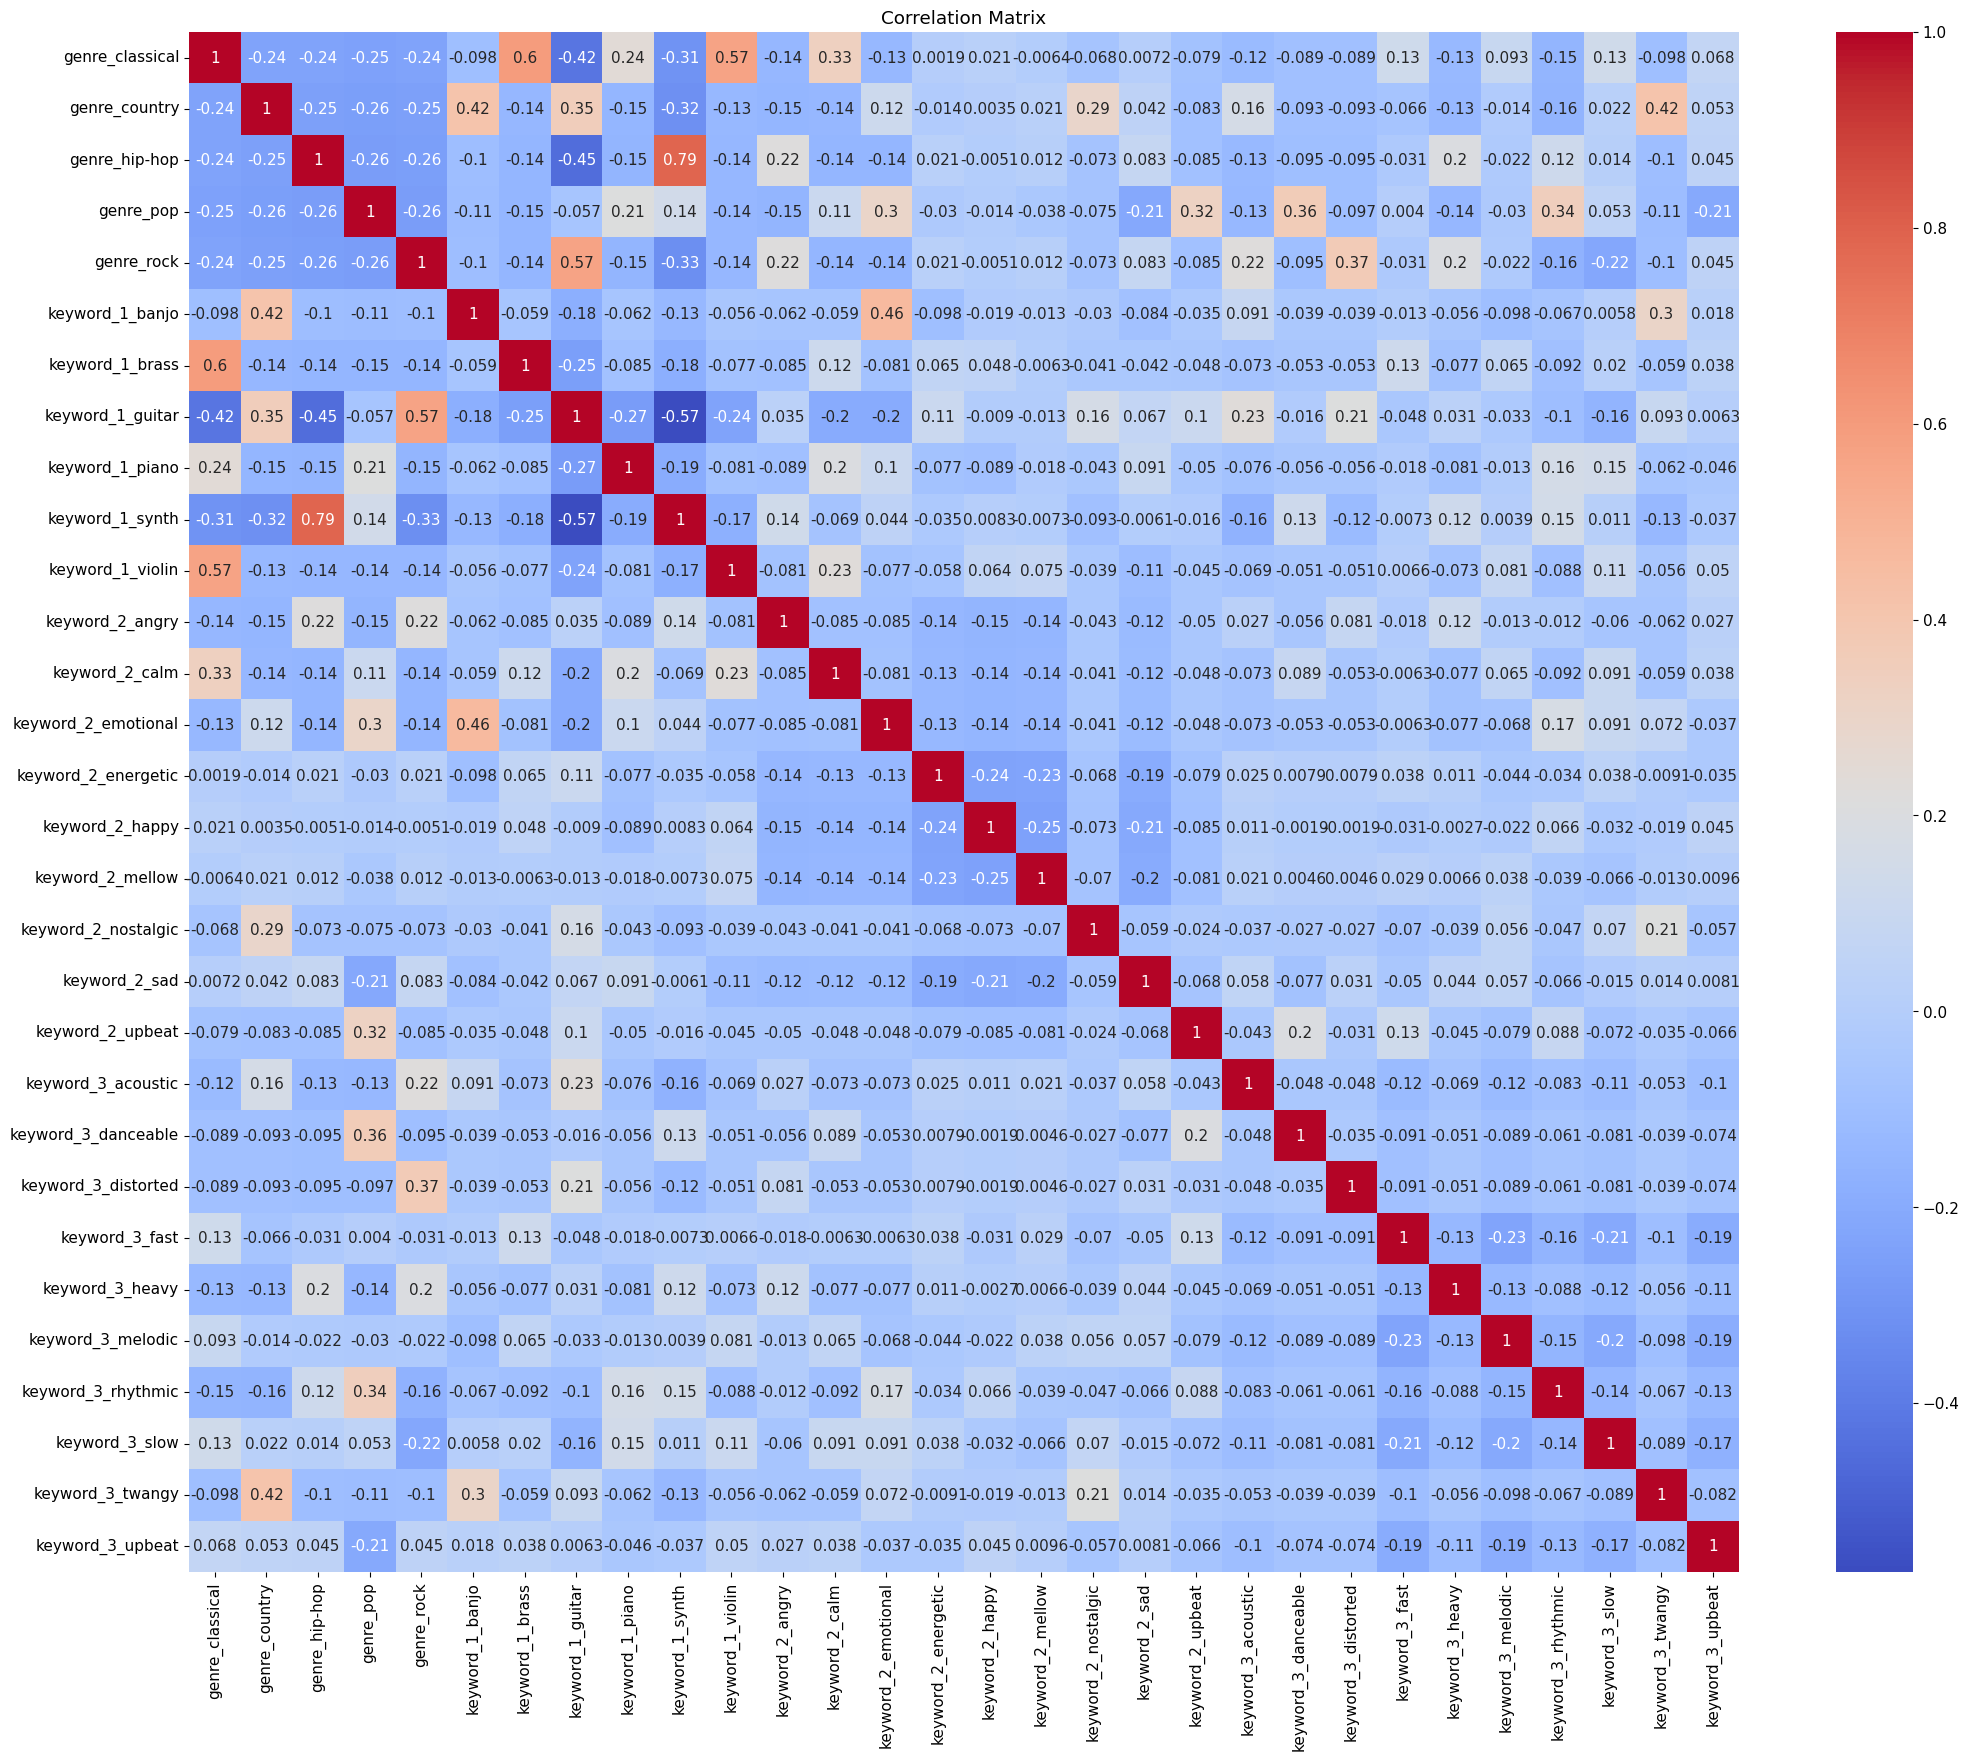
\includegraphics[width=300pt]{output8.png}
    \caption{Correlation Matrix for Keywords}
    \label{fig:correlation_matrix}
\end{figure}

\subsubsection{Analyzing the Keyword-Keyword Correlation}
\begin{itemize}
    \item The correlation matrix for the keywords brings out some interesting inferences. For example, 
\end{itemize}
\begin{figure}[h]
    \centering
    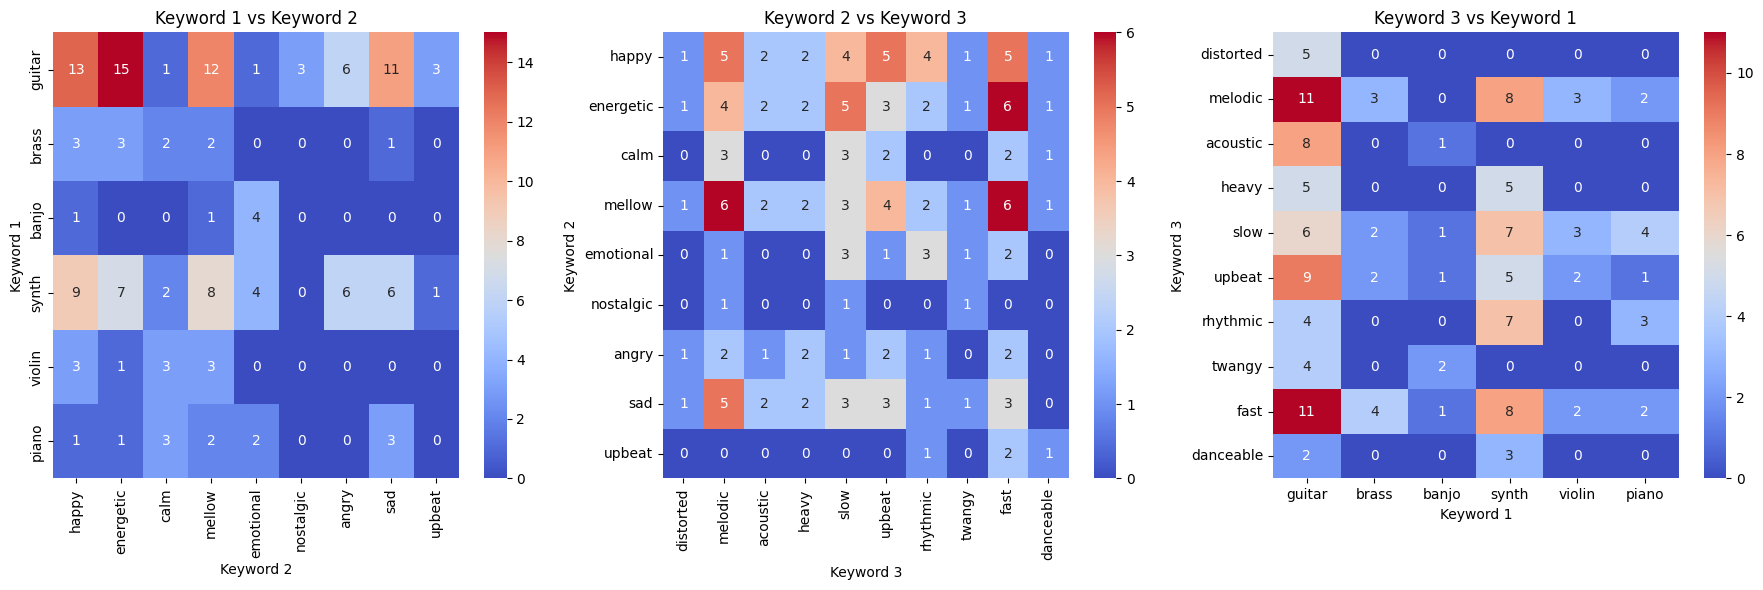
\includegraphics[width=300pt]{output9.png}
    \caption{Correlation Matrix for Keywords}
    \label{fig:correlation_matrix_keywords}
\end{figure}

\bibliographystyle{plain}
\bibliography{report}
\end{document}